\section{Results and Evaluation}

We evaluate VEXMLM using intrinsic tokenization quality metrics and extrinsic downstream task performance on Amharic and Tigrinya. All results are reported exactly as in the repository's result files and the released model cards: NER and SA accuracy and F1 as fractions with four decimals, QA Exact Match and F1 and the ablation accuracies as percentages with two decimals, and tokenizer metrics with four decimals. VEXMLM scores are means $\pm$ sample standard deviations over five seeds; differences are computed from unrounded means, as in the repository's tables, so they can differ by one unit in the last decimal from differences of the displayed values.

\subsection{Intrinsic Evaluation: Tokenization Quality}
Table~\ref{tab:tokenizer} compares the tokenizers of XLM-R, Glot500 and VEXMLM on the held-out Amharic and Tigrinya development sentences (\corpusAmhDev{} and \corpusTirDev{}). We do not report parity~\cite{petrov2023language}, which requires a sentence-aligned parallel corpus that was not available.

\begin{table}[t]
\centering
\scriptsize
\setlength{\tabcolsep}{4pt}
\begin{tabular}{llccc}
\toprule
\textbf{Metric} & \textbf{Language} & \textbf{XLM-R} & \textbf{Glot500} & \textbf{VEXMLM} \\
\midrule
\inputtable{generated/table_tokenizer.tex}
\bottomrule
\end{tabular}
\caption{Tokenizer metrics on held-out Amharic and Tigrinya text: fertility (tokens per word, lower is better), compression (characters per token, higher is better) and the share of OOV words (development-set words absent from the training lines) that the tokenizer reproduces exactly on decoding. Bold indicates the best fertility and compression. The XLM-R and VEXMLM columns come from \texttt{results/spmerge\_tokenizer\_metrics.json}; the Glot500 column comes from the earlier run \texttt{results/provenance/tokenizer\_metrics\_2026-08-15.json}, which measures the same development sets and reports identical XLM-R values. That earlier file also holds a superseded expanded-vocabulary variant, built with \texttt{add\_tokens} rather than SentencePiece merging, which is not the released model and is not reported here.}
\label{tab:tokenizer}
\end{table}

\paragraph{Fertility.} Fertility~\cite{rust2021good} measures the average number of tokens produced per input word; lower values indicate more efficient tokenization. Figure~\ref{fig:fertility} shows that VEXMLM achieves substantially lower fertility than XLM-R for Tigrinya (\tokXlmrTirFertility{} $\rightarrow$ \tokVexTirFertility, a \tokFertRedTir\% reduction) and Amharic (\tokXlmrAmhFertility{} $\rightarrow$ \tokVexAmhFertility, a \tokFertRedAmh\% reduction). Glot500 achieves intermediate fertility on both Ge'ez-script languages (\tokGlotAmhFertility{} and \tokGlotTirFertility). This reduction confirms that vocabulary expansion and integration effectively address the tokenization inefficiency observed in XLM-R for Ge'ez-script languages.

\begin{figure}[t]
\centering
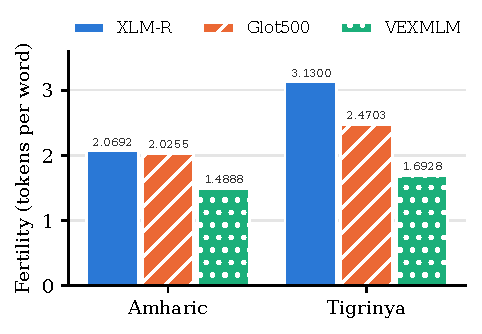
\includegraphics[width=\columnwidth]{generated/fig_fertility.pdf}
\caption{Fertility scores (tokens per word) for Amharic and Tigrinya. VEXMLM reduces fertility by \tokFertRedTir\% for Tigrinya and \tokFertRedAmh\% for Amharic relative to XLM-R.}
\label{fig:fertility}
\end{figure}

\paragraph{Compression.} Compression~\cite{goldman2024unpacking} measures characters per token; higher values indicate more efficient encoding. VEXMLM achieves higher compression for Amharic and Tigrinya than XLM-R and Glot500, in line with its fertility improvements. All three tokenizers reproduce nearly all OOV words exactly on decoding (Table~\ref{tab:tokenizer}).

\paragraph{Vocabulary coverage.} VEXMLM's vocabulary of \vocabFinal{} entries preserves all original XLM-R entries, so coverage for the 100 languages supported by the base model is unchanged.

\paragraph{OOV words.} Table~\ref{tab:oov} reports Tigrinya NER accuracy on OOV words (Section~\ref{sec:ablation_design}) and on all other words. VEXMLM improves accuracy by \oovGainTir{} points on OOV words and by \nonOOVGainTir{} points on the other words. For both models, accuracy on OOV words is higher than on the other words.

\begin{table}[t]
\centering
\scriptsize
\setlength{\tabcolsep}{3pt}
\begin{tabular}{lcccc}
\toprule
\textbf{Language} & \multicolumn{2}{c}{\textbf{XLM-R}} & \multicolumn{2}{c}{\textbf{VEXMLM}} \\
& Non-OOV & OOV & Non-OOV & OOV \\
\midrule
\inputtable{generated/table_oov.tex}
\bottomrule
\end{tabular}
\caption{Accuracy (\%) in Tigrinya NER (test split) on OOV words (Section~\ref{sec:ablation_design}) and on all other words (Non-OOV); mean $\pm$ standard deviation over five seeds.}
\label{tab:oov}
\end{table}

\subsection{Extrinsic Evaluation: Downstream Task Performance}
Table~\ref{tab:downstream} reports performance on all three downstream tasks. On NER, VEXMLM achieves higher accuracy than XLM-R on both MasakhaNER Amharic (\dsNERAmhDiff) and Tigrinya NER (\dsNERTirDiff), and higher macro-F1 on both (\appNERMacroFAmhDiff{} and \appNERMacroFTirDiff{}; Table~\ref{tab:appendix_f1}), larger margins than token accuracy shows; entity-level F1 is higher on Tigrinya (\appNEREntityFTirDiff) and comparable on Amharic, where the difference (\appNEREntityFAmhDiff) is within one standard deviation. On QA, VEXMLM scores below XLM-R on both datasets: by \dsQAEMAmhDiffAbs{} EM and \dsQAFoneAmhDiffAbs{} F1 points on AmQA, and by \dsQAEMTirDiffAbs{} EM and \dsQAFoneTirDiffAbs{} F1 points on TIGQA. On SA, the difference in accuracy (\dsSAAmhDiff) is within one standard deviation of VEXMLM's scores, so the two models are comparable. Because the XLM-R baseline is a single run, its own seed variance is unknown, and small differences should be read with caution.

\begin{table}[t]
\centering
\scriptsize
\setlength{\tabcolsep}{3pt}
\begin{tabular}{llcc}
\toprule
\textbf{Task (Metric)} & \textbf{Dataset} & \textbf{XLM-R}$^\ast$ & \textbf{VEXMLM} \\
\midrule
\inputtable{generated/table_downstream.tex}
\bottomrule
\end{tabular}
\caption{Downstream task performance. SA and NER report accuracy (fraction) on the test splits; QA reports Exact Match (EM) and F1 (\%) on the development splits. VEXMLM: mean $\pm$ standard deviation over five seeds. $^\ast$XLM-R: single run (seed 42). Bold marks the higher score where the difference exceeds one standard deviation of VEXMLM.}
\label{tab:downstream}
\end{table}

\subsection{Ablation Study}
\label{sec:ablation}
Table~\ref{tab:ablation} reports ablation results for Tigrinya NER OOV accuracy, isolating the contribution of each component. Vocabulary expansion with random initialization lowers this accuracy by \ablRandDeltaAbs{} points relative to the baseline; without continued pretraining, the new embedding rows receive no training before fine-tuning. Mean initialization recovers \ablMeanDeltaAbs{} points relative to random initialization. The full VEXMLM configuration (mean initialization + continued pretraining) achieves the best accuracy, with continued pretraining providing the largest single gain (\ablFullDeltaAbs{} points) and the full model finishing \ablFullVsBase{} points above the baseline. Updating the model's representations through MLM on Ge'ez-script corpora is therefore the most critical component of the pipeline. The configurations without continued pretraining also receive less training on Amharic and Tigrinya text, so part of this gain may reflect the additional training rather than the adaptation of the new embeddings; separating the two would require an unexpanded model given the same continued pretraining, which we did not run.

\begin{table}[t]
\centering
\scriptsize
\setlength{\tabcolsep}{4pt}
\begin{tabular}{lcc}
\toprule
\textbf{Configuration} & \textbf{OOV Acc.\ (\%)} & $\boldsymbol{\Delta}$ \\
\midrule
\inputtable{generated/table_ablation.tex}
\bottomrule
\end{tabular}
\caption{Ablation study: Tigrinya NER OOV accuracy under different configurations (mean $\pm$ standard deviation over five seeds). Rows 2 and 3 expand the vocabulary with random or mean initialization; row 4 adds continued pretraining to row 3; $\Delta$ is the change from the previous row, computed from unrounded means. Values as in the repository's \texttt{results/table5\_ablation.csv}.}
\label{tab:ablation}
\end{table}

\subsection{Discussion}
\label{sec:discussion}
The results show that VEXMLM's clearest improvement is in tokenization efficiency: targeted Ge'ez-script subword augmentation reduces fertility relative to XLM-R by \tokFertRedTir\% for Tigrinya and \tokFertRedAmh\% for Amharic, and yields lower fertility than Glot500 on both languages. The downstream effect of this efficiency depends on the task. On NER, VEXMLM improves over XLM-R, and the gain on Tigrinya holds for both OOV and other words. On extractive QA, VEXMLM scores below XLM-R on both datasets. The cause of this gap is not analysed in this work. On SA, the two models are comparable.

The ablation shows that vocabulary expansion by itself is harmful: new embeddings, whether random or mean-initialized, lower OOV accuracy until continued MLM pretraining adapts them. Mean initialization is a better starting point than random initialization, but the difference between them is small compared with the effect of continued pretraining.

Comparing with AfroXLMR and AfriBERTa is complicated by differing language coverage and evaluation protocols, and a direct, controlled comparison constitutes important future work. The 256-token sequence limit, under which long QA contexts are read in overlapping windows, may also constrain QA performance on long documents; future work should investigate full-length training.
